\chapter{Lecture 1: Sets and inequalities}
\section{Sets} \label{axioms}
A set \label{set} is a collection of objects, such as words or numbers. On its own, set theory is a powerful branch of mathematics. It can be used as a logical foundation onto which many (if not all) modern mathematical notions can be built. Some students may have heard of the `axioms of set theory,' or Zermelo-Fraenkel set theory. In some sense the goal of mathematics is to formulate simple assumptions (called axioms), and some rules governing how we interpret those assumptions, and then to essentially just `see' what follows from them. We have no need to dig into the formality of set theory here. \\

We will mostly be interested in sets containing things like
%THIS IS COPIED FROM LECTURE 1
\begin{itemize}
\item
the options available for some decision;
\item
the outcomes of a trial or experiment;
\item
the outcomes of a trial, with certain properties.
\end{itemize}
The objects that we put in a set are referred to as \textbf{elements} \label{element}. When writing a list of elements that belong to a set we place the elements inside set brackets \{ \}. \label{symbset} We can write, for example,
\[
A = \set{1,2,3,\text{set},\text{theory}}
\]
This means that $A$ is a set containing three numbers (1, 2 and 3), and two words (`set' and `theory'). \\

\noindent One of the most important things to remember about sets is that \textbf{repetition of the elements is not allowed.} So, the set $\set{1,1,2}$ is just the set $\set{1,2}$; or the set $\set{\text{`blue'},\text{'blue'}}$ is just the set $\set{\text{'blue'}}.$ Also, \textbf{it does not matter which order the elements are written in.} So, the set $\set{1,2,3}$ is equal to the set $\set{2,3,1}$; or the set  $\set{\text{`blue'},\text{'green'}}$ is equal to the set $\set{\text{`green'},\text{'blue'}}$\\


\noindent Another useful symbol is the `\textbf{such that}' symbol, which looks just like a colon~:~or sometimes a straight vertical bar $|$ \label{symbcolon} \label{symbmid}.

\subsection{Examples} \label{rational}
\begin{itemize}
\item
$A = \set{1,2,3,\ldots}$
\item
$B = \set{x \mid x \; \text{is a natural number}}$ \hspace{0.5cm} \textit{`the set of $x$ such that $x$ is a natural number.'}
\item
$C = \set{x \mid \text{$x$ is a whole number and $x$ is positive (and non-zero)}}$ \\ \\
Notice that $A,B,C$ are all the same set! We call this set the `natural numbers' \label{natural number} and denote it $\N$. \label{symbN} So $A = B = C = \N$.
\item
$D = \set{\ldots,-2,-1,\;0,\;1,\;2,\ldots}$
\item
$E = \set{x \mid \text{$x$ is an integer}}$ \hspace{1cm} \textit{`the set of $x$ such that $x$ is an integer.'} \\ \\
D and E are again equal to each other. They are referred to as the `integers,' \label{integer} denoted $\Z.$ \label{symbZ} This set, $\Z$, is an extension of $\N$ to include the negative whole numbers and zero.
\item
$F = \set{\displaystyle{\frac{p}{q}} \mid p,q \in \Z \;\; \text{and} \;\; q \neq 0}$ \\ \\ 
$F$ may look strange at first. $F$ is the set of fractions with a positive or negative whole number numerator and denominator. That is, F consists of fractions $\frac{p}{q}$ such that $p,q \in \Z$ but $q \neq 0$ (that is, $q$ is not equal to zero). \label{symbneq} This is actually a very familiar set; it is the set of all numbers that can be represented as whole number fractions. We refer to it as the set of rational numbers, \label{rational number} denoted $\Q$. \label{symbQ} We need the condition $q \neq 0$ since $q$ appears in the denominator, and division by zero is not defined (that is, not in standard axioms of mathematics!).
\end{itemize}



%--------------------------------------------------------------------------------Page 2 Sets and elements.
\section{Elements and subsets of sets}
We will need a few more useful pieces of notation with which to do probability. In particular, we want to be able to indicate when an element belongs to some set, and we also want to be able to indicate when one set is entirely contained within another set. \\ \\
Let's allow $X$ to represent the set of all letters of the alphabet. Clearly the letter $a$ belongs to $X$, and also the letter $b$, and so on all the way to $z$. We use the symbol $\in$ to show that an element belongs to a set; to show that $a$ belongs to $X$, we write \label{symbin}
	
	\bigskip
	
	\hfil\fbox{
	\begin{minipage}{0.1\columnwidth}{
	
	\vskip 0.02cm
	\begin{center}
	$a \in X$
	\end{center}
	}
	\end{minipage}}
	\bigskip

\noindent If every element of one set, say $Y$, is also an element of $X$, then we say ``$Y$ is a subset of $X$''. For example, if $Y = \set{a,b,c,d}$, then for any $x \in Y$ we know that $x \in X$ also (since $X$ is the set of all letters of the alphabet). To indicate that $Y$ is a subset of $X$ we write \label{symbsubseteq} \label{subset}
	\bigskip
	
	\hfil\fbox{
	\begin{minipage}{0.1\columnwidth}{
	
	\vskip 0.02cm
	\begin{center}
	$Y \subseteq X$
	\end{center}
	}
	\end{minipage}}
	\bigskip

\noindent How do we know when two sets are equal? Suppose we have another set $P = \set{a,b,c,\ldots,z}$, that also contains all the letters of the alphabet (and nothing more). Then every element of $P$ is also in $X$ so we can write $P \subseteq X$. Furthermore, every element of $X$ is contained in $P$, so we can write $X \subseteq P$. When $X \subseteq P$ and $P \subseteq X$ we can write $P = X$, meaning that $P$ and $X$ are equal. \\ \\
Suppose we have an element which does not belong to $X$. Take for example the word `hello'. This word, `hello,' does not belong to the alphabet. To indicate that `hello' is not an element of $X$ we write  \label{symbnotin}
	\bigskip
	
	\hfil\fbox{
	\begin{minipage}{0.18\columnwidth}{
	
	\vskip 0.02cm
	\begin{center}
	$\text{`hello'} \notin X$
	\end{center}
	}
	\end{minipage}}
	\bigskip

\noindent Similarly, if we have a set $Q$ that has at least one element that is not contained in $X$, then $Q$ is not a subset of $X$. We may have $Q = \set{a,b,c,d,(1,5)}.$ The element $(1,5)$ is an element of $Q$ but it is not an element of $X$. That is $(1,5) \in Q$ and $(1,5) \notin X$. Therefore $Q$ is not a subset of $X$, so we write \label{symbnotsubseteq}
	\bigskip
	
	\hfil\fbox{
	\begin{minipage}{0.18\columnwidth}{
	
	\vskip 0.02cm
	\begin{center}
	$Q \not\subseteq X$
	\end{center}
	}
	\end{minipage}}
	\bigskip

\noindent Notice a subtle property of the notation we have just introduced: The $\in$ symbol and the $\subseteq$ symbol (along with their logical negations $\notin$ and $\not\subseteq$), are all written with one symbol on either side (two symbols in total), so that we write for example $\mathbf{a} \in X$ and $\mathbf{Y} \subseteq Q$. Take a moment to compare the symbols $\mathbf{a}$ and $\textbf{Y}$ to each other. The symbol $Y$ has been used to represent a set $Y = \set{a,b,c,d}$; whereas the symbol $a$ was only used to represent a single element. We must be careful to remember that $a \neq \set{a}$. That is, the \textbf{element} $a$ does not equal the set containing the element $a$. In the case of our example it is perfectly true to write $a \not\subseteq X$ and $Y \notin X$.  \\ \\
We have one final useful piece of notation to introduce for this section. Consider the set $\set{}$. This is the set containing no elements. This idea is similar to the number 0. We call this the empty set, \label{empty set} and we denote it $\varnothing$. \label{symbvarnothing} That is,
	\bigskip
	
	\hfil\fbox{
	\begin{minipage}{0.18\columnwidth}{
	
	\vskip 0.02cm
	\begin{center}
	$\set{} = \varnothing$
	\end{center}
	}
	\end{minipage}}
	\bigskip

%-------------------------------------------------------------------------Page 3: Intersections, unions, and compliments of sets.

\section{Universal set, complements, intersections and unions}
%THIS IS COPIED FROM LECTURE 1
We will soon see that it will be necessary for us to have a well defined collection of all possible outcomes of an experiment or trial when we are working with probabilities. We call this collection the universal set. It is denoted $\Omega$ \label{symbOmega} (this is the Greek letter `Omega'). Thus, for the purpose of probabilities \label{omega}\label{universal set}
	\bigskip
	
	\hfil\fbox{
	\begin{minipage}{0.4\columnwidth}{
	
	\vskip 0.02cm
	\begin{center}
	$\Omega = \set{x \mid \text{$x$ is a possible outcome}}$
	\end{center}
	}
	\end{minipage}}
	\bigskip

\noindent More generally, choosing $\Omega$ gives us a firm understanding of the collection of all elements that we are taking into consideration. Suppose you have decided on a set $\Omega$, and have chosen some subset $A$ containing some of the possible outcomes (i.e., $A \subseteq \Omega$). Then it is natural to think about all of the things in $\Omega$ that are not in $A$. That is, it is natural to think about the set~$\set{x \in \Omega \mid x \notin A}$. We call this set the complement \label{complement} of $A$ and we denote it $A^c$ \label{symbcomplement} or sometimes $A'$. So that
	\bigskip
	
	\hfil\fbox{
	\begin{minipage}{0.3\columnwidth}{
	
	\vskip 0.02cm
	\begin{center}
	$A^c = \set{x \in \Omega \mid x \notin A}$
	\end{center}
	}
	\end{minipage}}
	\bigskip

\noindent It reads, \textit{`the set of $x$ belonging to omega, such that $x$ is not an element of $A.$'} \\ \\
These ideas are perhaps best illustrated with Venn Diagrams. 
	\begin{figure}[h!]
	\centering
	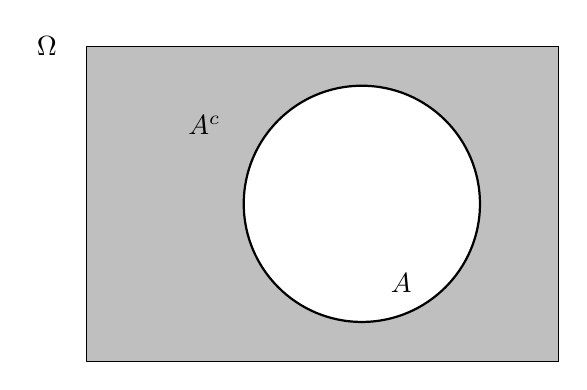
\begin{tikzpicture}
	\draw [fill = lightgray] (-3,-2) -- (-3,2) -- (3,2) -- (3,-2) -- cycle;
	%\draw [fill = white] (-0.5,0.8) ellipse (1.6cm and 0.8cm);
	\draw [thick, fill = white] (0.5,0) circle (1.5);
	%\draw [thick] (-0.5,0.8) ellipse (1.6cm and 0.8cm);
	\draw (1,-1) node {$A$};
	\draw (-3.5,2) node {$\Omega$};
	\draw (-1.5,1) node {$A^c$};
	\end{tikzpicture}
	%\caption{Venn Diagram of $A$ and $A^c.$}
	\end{figure}

\noindent In the diagram, the white circle represents $A$, the gray area represents $A^c$, and the whole square is $\Omega$. Notice that $A$ and $A^c$ together make up $\Omega$. For any two sets $A$, $B$, we define the union \label{union} of $A$ and $B$ to be the set containing every element from $A$ and every element from $B$. We write $A \cup B$. \label{symbcup} So in other words
	\bigskip
	
	\hfil\fbox{
	\begin{minipage}{0.4\columnwidth}{
	
	\vskip 0.02cm
	\begin{center}
	$A \cup B = \set{x \mid x \in A \; \text{or} \; x \in B}$
	\end{center}
	}
	\end{minipage}}
	\bigskip
 
We have noticed that

	\bigskip
	
	\hfil\fbox{
	\begin{minipage}{0.2\columnwidth}{
	
	\vskip 0.02cm
	\begin{center}
	$\Omega = A \cup A^c$
	\end{center}
	}
	\end{minipage}}
	\bigskip


%-----------------------------------------page 4 ---------------- continued

Consider the following Venn Diagram
	\begin{figure}[h!]
	\centering
	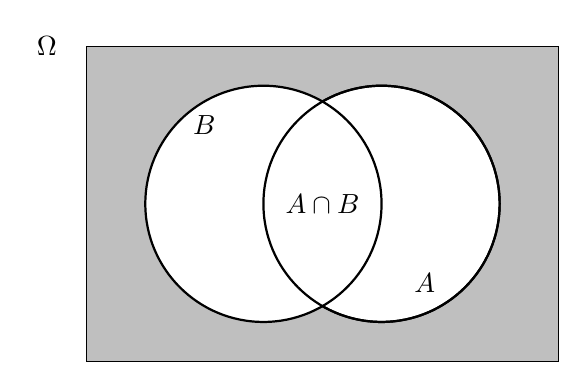
\begin{tikzpicture}
	\draw [fill = lightgray] (-3,-2) -- (-3,2) -- (3,2) -- (3,-2) -- cycle;
	%\draw [fill = white] (-0.5,0.8) ellipse (1.6cm and 0.8cm);
	\draw [thick, fill = white] (0.75,0) circle (1.5);
	\draw [thick, fill = white] (-0.75,0) circle (1.5);
	\draw [thick] (0.75,0) circle (1.5);
	%\draw [thick] (-0.5,0.8) ellipse (1.6cm and 0.8cm);
	\draw (1.3,-1) node {$A$};
	\draw (-3.5,2) node {$\Omega$};
	\draw (-1.5,1) node {$B$};
	\draw (0,0) node {$A \cap B$};
	\end{tikzpicture}
	%\caption{Venn Diagram of $A$ and $A^c.$}
	\end{figure}

For any two sets $A,B$ we define the intersection \label{intersection} $A \cap B$ to be the set containing only those elements that are shared by $A$ and $B$. We denote this set $A \cap B$. Formally, \label{symbcap}
\bigskip

\hfil\fbox{
\begin{minipage}{0.4\columnwidth}{

\vskip 0.02cm
\begin{center}
$A \cap B = \set{x \mid x \in A \; \text{and} \; x \in B}$
\end{center}
}
\end{minipage}}
\bigskip

Notice the difference between our definitions of union and intersection inside the boxes. The only difference was in the use of the word `\textit{or}' in the definition of union versus the use of the word `\textit{and}' in the definition of intersection. This subtlety is a useful way to remember the definitions themselves. It is also an interesting property of these two words. \\ \\

\noindent One highly important idea relating to intersections is the notion of \textbf{disjoint} \label{disjoint} sets, sometimes referred to as \textbf{mutually exclusive} sets. \label{mutually exclusive} Informally, disjoint sets are those which do not overlap on a Venn Diagram. In other words, two sets $A,B$ are disjoint if $A$ and $B$ have an empty intersection; that is,
\bigskip

\hfil\fbox{
\begin{minipage}{0.4\columnwidth}{

\vskip 0.02cm
\begin{center}
$A$ and $B$ are disjoint if $A \cap B = \varnothing$
\end{center}
}
\end{minipage}}
\bigskip

\noindent On a Venn Diagram, disjoint sets $A$ and $B$ would appear as follows

	\begin{figure}[h!]
	\centering
	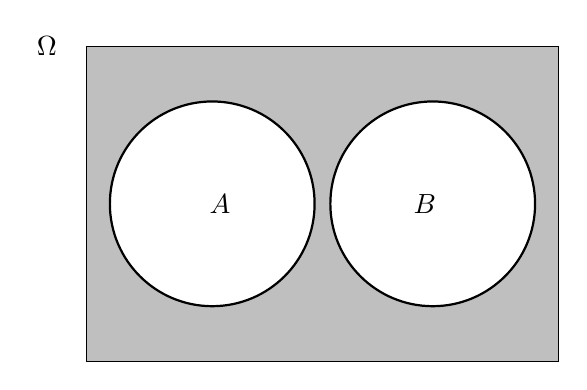
\begin{tikzpicture}
	\draw [fill = lightgray] (-3,-2) -- (-3,2) -- (3,2) -- (3,-2) -- cycle;
	%\draw [fill = white] (-0.5,0.8) ellipse (1.6cm and 0.8cm);
	\draw [thick, fill = white] (1.4,0) circle (1.3);
	\draw [thick, fill = white] (-1.4,0) circle (1.3);
	%\draw [thick] (1.4,0) circle (1.5);
	%\draw [thick] (-0.5,0.8) ellipse (1.6cm and 0.8cm);
	\draw (1.3,0) node {$B$};
	\draw (-3.5,2) node {$\Omega$};
	\draw (-1.3,0) node {$A$};
	%\draw (0,0) node {$A \cap B$};
	\end{tikzpicture}
	%\caption{Venn Diagram of $A$ and $A^c.$}
	\end{figure}


%----------------------------------------------------------------------------------------Page 5
\newpage
\section{Some very useful properties of sets} \label{setproperties1}
These properties will definitely come in handy while working with probabilities. We introduce them first on face value, then in the examples section below we will get an idea of why they are true. It is a great idea to memorise them; notice in each case where there are a pair of properties labelled (i) and (ii), that property (ii) is obtained from property (i) simply by switching every instance of $\cup$ for $\cap$, and every instance of $\cap$ for $\cup$. \\ \\
For any sets $A,B,C$ the following hold
\begin{itemize}
	\item \textbf{The inclusion-exclusion principle} \label{inclusion-exclusion principle} \\
	Size of $A \cup B$ = size of $A$ + size of $B$ - size of $A \cap B$.
	\item \textbf{De Morgan's Laws} \label{de-morgans laws} \\
	(i)\;\;\;$\brac{A \cup C}^c = A^c \cap C^c$ \\
	(ii)\;\;$\brac{A \cap C}^c = A^c \cup C^c$
	\item \textbf{Distributive Laws} \label{distributive law} \\
	(i)\;\;\;$\brac{A \cup C} \cap B = (A \cap B) \cup (C \cap B)$ \\
	(ii)\;\;$\brac{A \cap C} \cup B = (A \cup B) \cap (C \cup B)$
	\item \textbf{Commutative Laws} \label{commutative law} \\
	(i)\;\;\;$A \cup B = B \cup A$ \\
	(ii)\;\;$A \cap B = B \cap A$
	\item \textbf{Associative Laws} \label{associative law} \\
	(i)\;\;\; $(A \cup B) \cup C = A \cup (B \cup C)$ \\
	(ii)\;\; $(A \cap B) \cap C = A \cap (B \cap C)$
	\item \textbf{More properties} \label{more properties} \\
	- \;\;\; $A \cup A^c = \Omega$ \\
	- \;\;\; $A \cap A^c = \varnothing$ \\
	- \;\;\; $A \cup \varnothing = A$ \\
	- \;\;\; $A \cap \varnothing = \varnothing$
\end{itemize}



\subsection{Examples}
	
	\begin{figure}[h!]
	\centering
	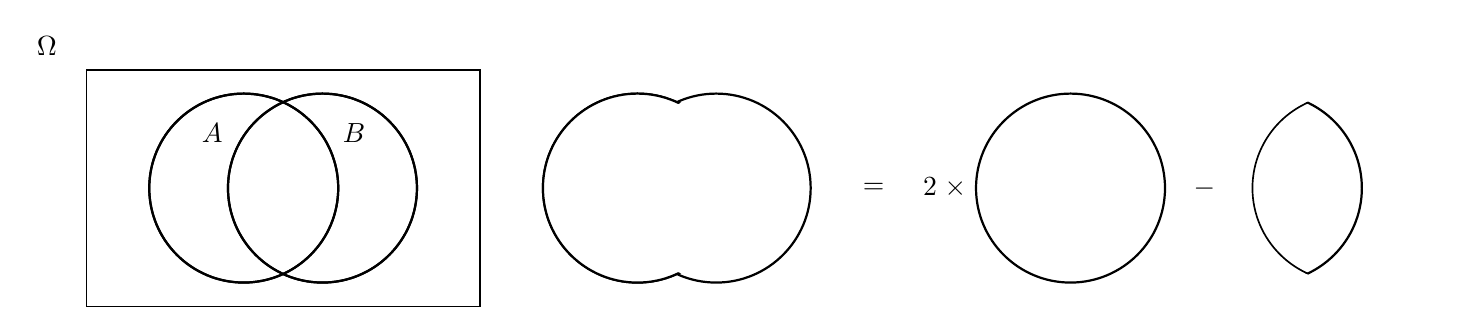
\begin{tikzpicture} [fill = white]
	\draw (-2.5,-1.5) -- (-2.5,1.5) -- (2.5,1.5) -- (2.5,-1.5) -- cycle;
	%\draw [fill = white] (-0.5,0.8) ellipse (1.6cm and 0.8cm);
	\draw [thick] (0.5,0) circle (1.2); %B
	\draw [thick] (-0.5,0) circle (1.2); %A
	%\draw [thick, fill = white] (0,-0.5) circle (1.3); %C
	\draw [thick] (0.5,0) circle (1.2); %B
	\draw [thick] (-0.5,0) circle (1.2); %A
	%\draw [thick] (0,-0.5) circle (1.3); %C
	%\draw [thick] (1.4,0) circle (1.5);
	%\draw [thick] (-0.5,0.8) ellipse (1.6cm and 0.8cm);
	\draw (0.9,0.7) node {$B$};
	\draw (-3,1.8) node {$\Omega$};
	\draw (-0.9,0.7) node {$A$};
	%\draw (0,-1.2) node {$C$};
	%\draw (0,0) node {$A \cap B$};
	\draw [thick] (5.5,0) circle (1.2); %B
	\draw [thick] (4.5,0) circle (1.2); %A
	\draw [thick, fill = white] (4.5,0) circle (1.2);
	\scope 
	\clip (5.5,0) circle (1.2);
	\fill (5.5,0) circle (1.17);
	\endscope
	\draw (7.5,0) node {$=$}; 
	\draw (8.4,0) node {$2\;\times$};
	\draw [thick] (10,0) circle (1.2);
	\draw (11.7,0) node {$-$};
	\scope
	\clip (13.5,0) circle (1.2); %B
	\draw [thick] (12.5,0) circle (1.2); %A
	\clip (12.5,0) circle (1.2); %A
	\draw [very thick](13.5,0) circle (1.2); %B
	\endscope
	\end{tikzpicture}
	\caption*{Size of $A \cup B =$ size of $A$ + size of $B$ - size of $A \cap B$}
	\end{figure}
	
%----------------------------------------------------------------------------------------Page 6	
	\begin{figure}[h!]
	\centering
	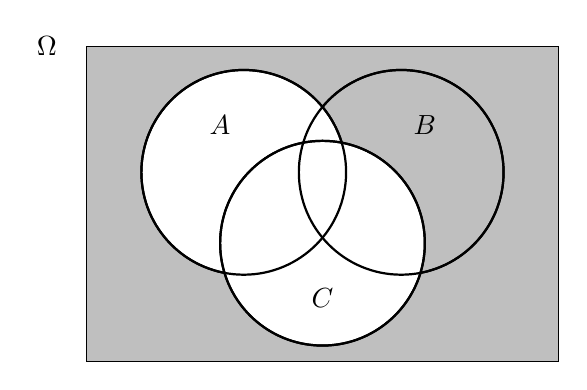
\begin{tikzpicture}
	\draw [fill = lightgray] (-3,-2) -- (-3,2) -- (3,2) -- (3,-2) -- cycle;
	%\draw [fill = white] (-0.5,0.8) ellipse (1.6cm and 0.8cm);
	\draw [thick, fill = lightgray] (1,0.4) circle (1.3);
	\draw [thick, fill = white] (-1,0.4) circle (1.3);
	\draw [thick, fill = white] (0,-0.5) circle (1.3);
	\draw [thick] (1,0.4) circle (1.3);
	\draw [thick] (-1,0.4) circle (1.3);
	\draw [thick] (0,-0.5) circle (1.3);
	%\draw [thick] (1.4,0) circle (1.5);
	%\draw [thick] (-0.5,0.8) ellipse (1.6cm and 0.8cm);
	\draw (1.3,1) node {$B$};
	\draw (-3.5,2) node {$\Omega$};
	\draw (-1.3,1) node {$A$};
	\draw (0,-1.2) node {$C$};
	%\draw (0,0) node {$A \cap B$};
	\end{tikzpicture}
	\caption*{The shaded area represents both $(A \cup C)^c$ and $A^c \cap C^c$}
	\end{figure}
	
	\begin{figure}[h!]
	\centering
	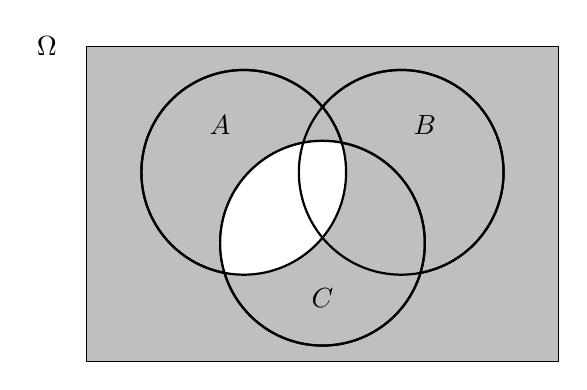
\begin{tikzpicture} [fill = white]
	\draw [fill = lightgray] (-3,-2) -- (-3,2) -- (3,2) -- (3,-2) -- cycle;
	%\draw [fill = white] (-0.5,0.8) ellipse (1.6cm and 0.8cm);
	\draw [thick, fill = lightgray] (1,0.4) circle (1.3);
	\draw [thick, fill = lightgray] (-1,0.4) circle (1.3);
	\draw [thick, fill = lightgray] (0,-0.5) circle (1.3);
	\scope
	\clip (0,-0.5) circle (1.3);
	\fill (-1,0.4) circle (1.3);
	\endscope
	\draw [thick] (1,0.4) circle (1.3);
	\draw [thick] (-1,0.4) circle (1.3);
	\draw [thick] (0,-0.5) circle (1.3);
	%\draw [thick] (1.4,0) circle (1.5);
	%\draw [thick] (-0.5,0.8) ellipse (1.6cm and 0.8cm);
	\draw (1.3,1) node {$B$};
	\draw (-3.5,2) node {$\Omega$};
	\draw (-1.3,1) node {$A$};
	\draw (0,-1.2) node {$C$};
	%\draw (0,0) node {$A \cap B$};
	\end{tikzpicture}
	\caption*{The shaded area represents both $(A \cap C)^c$ and $A^c \cup C^c$}
	\end{figure}
	
	\begin{figure}[h!]
	\centering
	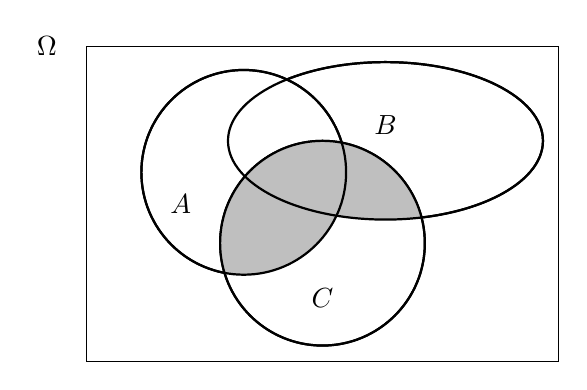
\begin{tikzpicture}[fill = lightgray]
	\draw (-3,-2) -- (-3,2) -- (3,2) -- (3,-2) -- cycle;
	%\draw [fill = white] (-0.5,0.8) ellipse (1.6cm and 0.8cm);
	%\draw [thick, fill = lightgray] (1,0.4) circle (1.3);
	\draw [thick,fill = white] (0.8,0.8) ellipse (2cm and 1cm);
	\draw [thick, fill = white] (-1,0.4) circle (1.3);
	\draw [thick, fill = white] (0,-0.5) circle (1.3);
	\scope
	\clip (0,-0.5) circle (1.3);
	\fill (0.8,0.8) ellipse (2cm and 1cm);
	\fill (-1,0.4) circle (1.3);
	\endscope
	%\draw [thick] (1,0.4) circle (1.3);
	\draw [thick] (-1,0.4) circle (1.3);
	\draw [thick] (0,-0.5) circle (1.3);
	%\draw [thick] (1.4,0) circle (1.5);
	\draw [thick] (0.8,0.8) ellipse (2cm and 1cm);
	\draw (0.8,1) node {$B$};
	\draw (-3.5,2) node {$\Omega$};
	\draw (-1.8,0) node {$A$};
	\draw (0,-1.2) node {$C$};
	%\draw (0,0) node {$A \cap B$};
	\end{tikzpicture}
	\caption*{The shaded area represents both $(B \cup A) \cap C$ and $(B \cap C) \cup (A \cap C)$}
	\end{figure}
	
	
	\begin{figure}[h!]
	\centering
	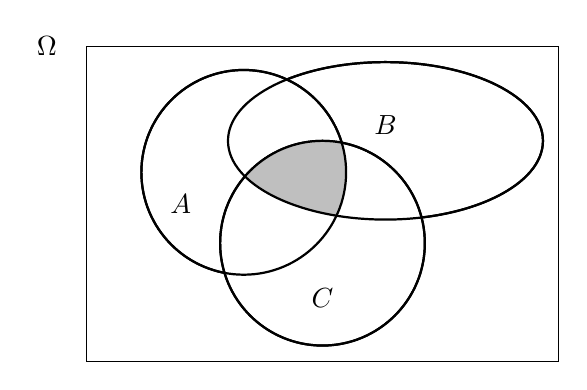
\begin{tikzpicture}[fill = lightgray]
	\draw (-3,-2) -- (-3,2) -- (3,2) -- (3,-2) -- cycle;
	%\draw [fill = white] (-0.5,0.8) ellipse (1.6cm and 0.8cm);
	%\draw [thick, fill = lightgray] (1,0.4) circle (1.3);
	\draw [thick,fill = white] (0.8,0.8) ellipse (2cm and 1cm);
	\draw [thick, fill = white] (-1,0.4) circle (1.3);
	\draw [thick, fill = white] (0,-0.5) circle (1.3);
	\scope
	\clip (0.8,0.8) ellipse (2cm and 1cm);
	\clip (0,-0.5) circle (1.3);
	\fill (-1,0.4) circle (1.3);
	\endscope
	%\draw [thick] (1,0.4) circle (1.3);
	\draw [thick] (-1,0.4) circle (1.3);
	\draw [thick] (0,-0.5) circle (1.3);
	%\draw [thick] (1.4,0) circle (1.5);
	\draw [thick] (0.8,0.8) ellipse (2cm and 1cm);
	\draw (0.8,1) node {$B$};
	\draw (-3.5,2) node {$\Omega$};
	\draw (-1.8,0) node {$A$};
	\draw (0,-1.2) node {$C$};
	%\draw (0,0) node {$A \cap B$};
	\end{tikzpicture}
	\caption*{The shaded area represents both $(B \cap A) \cap C$ and $B \cap (A \cap C)$}
	\end{figure}


%-----------------------------------------------------------------------------Page 7
\newpage
\phantom{h}
\newpage
\section{Inequalities}
An \textbf{equality} \label{equality} is a statement consisting of two mathematical expressions, separated by the `$=$' symbol. An \textbf{inequality} \label{inequality} is, similarly, a pair of mathematical expressions; however the expressions in an inequality are separated by one of the following symbols \label{symbinequalities}
\[
\geq \qquad > \qquad \leq \qquad < 
\]
Inequalities tell us about the \textbf{ordering} \label{order} relationship between two mathematical expressions. When we have two expressions $\mathcal{A}$ and $\mathcal{B}$, which have some rules governing their order with respect to one another, we can write
\begin{itemize}
\item $\mathcal{A} \geq \mathcal{B}$ \qquad \textit{`$\mathcal{A}$ is greater than or equal to $\mathcal{B}$'}
\item $\mathcal{A} > \mathcal{B}$ \qquad \textit{`$\mathcal{A}$ is (strictly) greater than $\mathcal{B}$'}
\item $\mathcal{A} \leq \mathcal{B}$ \qquad \textit{`$\mathcal{A}$ is less than or equal to $\mathcal{B}$'}
\item $\mathcal{A} < \mathcal{B}$ \qquad \textit{`$\mathcal{A}$ is (strictly) less than $\mathcal{B}$'}
\end{itemize}

\subsection{Examples} \label{dot}
\begin{itemize}
\item
The \textbf{real numbers} \label{real numbers} form the set of all numbers that we are used to using in every day life. We denote this set $\R.$ \label{symbR} It includes all the numbers from $\Q$ (the rational numbers, see example \ref{rational}), along with all the irrational numbers. The irrational numbers, \label{irrational numbers} like $\sqrt{2}$ or $\pi$, cannot be represented as fractions with integer numerator and denominator so they are not members of the set $\Q$ of rational numbers; this is why we call them irrational. For our purposes, we can just think of the real numbers as the set containing every number we would ever want to use. We can very intuitively understand the ordering relationship between real numbers, for example we can organise the numbers $\frac{3}{4}, 2, 0.8, 0.75,$ and $\sqrt{7}$ in order as follows,
\[
0.75 \leq \frac{3}{4} < 0.8 < 2 < \sqrt{7}
\]
Notice that we write $0.75 \leq \frac{3}{4}$. We could also write it the other way as $\frac{3}{4} \leq 0.75$. This is because in the case of $0.75$ and $\frac{3}{4}$ we have $0.75 = \frac{3}{4}$. So they are both `less than or equal to' each other (because they are equal to each other).
\item
We can now write sets like $\set{x \in \R \mid x > \pi}$; this is the set of $x$ belonging to $\R$ such that $x$ is strictly greater than $\pi.$ This set does not include $\pi$, but it includes every real number greater than $\pi$. For example it includes $\pi + 1$, or $\pi + 1/2$ or even $\pi + 0.00000000001$. In fact, if we pick any number greater than $\pi$, no matter how small it is, we can still find a smaller number that is also strictly greater than $\pi$ (just by halving the distance to $\pi$ each time). 
\item
We can also use the ordering from other sets, e.g., $\N$ or $\Z,$ that we introduced in example~\ref{rational}.
\begin{itemize}
\item
$\set{x \in \N \mid 2 \leq x \leq 4} = \set{2,3,4}$
\item
 $\set{x \in \N \mid x \leq 4} = \set{1,2,3,4}$
\item
 $\set{x \in \N \mid x < 4} = \set{1,2,3}$
\item
 $\set{x \in \N \mid x < \frac{7}{2}} = \set{1,2,3}$
\item
 $\set{x \in \N \mid x > \sqrt{2}} = \set{2,3,4,\ldots}$
\item
 $\set{x \in \Z \mid x < 4} = \set{\ldots,-3,-2,-1,0,1,2,3}$ 
\end{itemize}
\end{itemize}

%----------------------------------------------------------------Page 8

\subsection{Intervals}
Notice in the first dot point of the last example from examples \ref{dot} we wrote \\ the set $\set{x \in \N \mid 2 \leq x \leq 4}$. Sets of this form are called \textbf{intervals}. \label{intervals} When writing intervals from $\N$ or from $\Z$ we usually write them with set brackets, for example $\set{x \in \Z \mid a \leq x < b}$ for some real numbers $a$ and $b$. The set in this example includes $a$ but does not include $b$; however, any arrangement of $\geq\;, >,\; \leq,\; <$ can be used. We need to be careful though; for example the set $\set{x \in \N \mid 3 > x < 2}$ is much better written $\set{x \in \N \mid x < 2}$ and the set $\set{x \in \N \mid 4 < x < 2}$ is empty, because there are no elements of $\N$ which are greater than 4 yet less than 2. \\

\noindent The real interval $\set{x \in \R \mid 0 \leq x \leq 1}$ can simply be written $0 \leq x \leq 1$ for convenience. However, there is a very common, much simpler convention for writing \textbf{real number intervals}, which is sometimes referred to as \textbf{interval notation} (though we need to be careful to remember that interval notation can only be used for real number intervals, and not for intervals in sets like $\Z$ or $\N$): The real interval ``$0 \leq x \leq 1$'' is written in interval notation simply as ``$[0,1]$''. For the real interval $\sqrt{2} < x < 4$ we write $(\sqrt{2},4).$ We use square brackets [, ] \label{symbinterval} to indicate that the interval includes its boundary (i.e., to indicate ``$\leq$''), and round brackets to indicate that it does not (i.e., to indicate ``$<$''). For example, the set $[1,3)$ includes 1, and it includes all of the real numbers from 1 to 3, but it excludes 3. We will give a better description of interval notation in section~\ref{interval notation}. \label{interval notation 1}


\subsection{Three rules for rearranging inequalities} \label{secinecrule}
%---STRAIGHT FROM THE SLIDES
\begin{enumerate}
\item
If you add or subtract the same number from each side, the direction of the inequality does not change.
\item
If you multiply each side by the same \textbf{positive} number, the direction of the inequality does not change.
\item
If you multiply each side by the same \textbf{negative} number, the direction of the inequality is \textbf{reversed}.
\end{enumerate}
\subsection{Example}
Let $p \in [-10,0)$ (i.e., let $p$ be a real number between -10 and 0, not including 0) and suppose~that~$p~<~3p^2~+~p^3 + p.$ We can simplify this inequality using rules 1 to 3. We have,
\begin{alignat*}{2}
&& p
& < 3p^2 + p^3 + p \\
&\iff 
& 0 
& < 3p^2 + p^3 \tag{subtracting $p$ from both sides (applying rule 1)} \\
&\iff 
& -p^3 
& < 3p^2 \tag{again, using rule 1 (subtracting $p^3$ from both sides)} \\
& \iff 
& \frac{-p^3}{p^2} 
& < \frac{3p^2}{p^2} \tag{dividing by $p^2$ (rule 2 since $p \in (0,1]$ so $p^2$ must be positive)} \\
& \iff
& -p 
& < 3 \tag{using simple algebra of fractions} \\
& \iff
& (-1)\times(-p) 
& > (-1)\times3 \tag{rule 3 (multiplying by a \textbf{negative} number)} \\
& \iff
& p
& > -3
\end{alignat*}
Notice that in the final step the direction of the inequality changed by rule 3. Also notice that when we divided by $p^2$ we had to be sure that $p^2 \neq 0$; since $p \in [-10,0)$ we know that $p$ is not equal to zero, so $p^2$ must not be equal to zero either (if you multiply two non-zero numbers you always get a non-zero number). Always be careful not to divide by zero!

\subsection{Example}
Sometimes the following result is taken as an extra rule. However, it is just a consequence of rules 2 and 3. We will show this now. \\
Let $a,b$ be non-zero real numbers that are \textbf{both positive}. Then
\begin{alignat*}{2}
&& a 
& \geq b \\
& \iff 
& 1
& \geq \frac{b}{a} \tag{multiplying both sides by $\frac{1}{a},$ (using rule 2, as $a$ is positive)} \\
& \iff
& \frac{1}{b}
& \geq \frac{b}{ab} \tag{multiplying both sides by $\frac{1}{b},$ (using rule 2, as $b$ is positive)} \\
& \iff
& \frac{1}{b}
& \geq \frac{1}{a} \tag{using simple algebra of fractions}
\end{alignat*}
Suppose instead that $a,b$ are non-zero real numbers that are \textbf{both negative}. Then
\begin{alignat*}{2}
&& a 
& \geq b \\
& \iff 
& 1
& \leq \frac{b}{a} \tag{multiplying both sides by $\frac{1}{a},$ (using rule 3, as $a$ is negative)} \\
& \iff
& \frac{1}{b}
& \geq \frac{b}{ab} \tag{multiplying both sides by $\frac{1}{b},$ (using rule 3, as $b$ is negative)} \\
& \iff
& \frac{1}{b}
& \geq \frac{1}{a} \tag{using simple algebra of fractions}
\end{alignat*}
In both cases we conclude that if $a,b$ are \textbf{both positive} or if $a,b$ are \textbf{both negative} then 
\[
a \geq b \iff \frac{1}{b} \geq \frac{1}{a}
\]
Again, be sure to check that $a$ and $b$ are both non-zero so as not to divide by zero (it is surprisingly easy to do when working with variables).

\subsection*{Dividing by zero}
Here is a great example of the kind of zany results we can achieve if we accidentally divide by zero. Firstly, suppose we have two variables, $a,b$ such that $\textbf{a = b}.$ Then
\begin{alignat*}{2}
&& a 
& = b \\
&\iff
&ab 
& = b^2 \tag{multiplying both sides by $b$} \\
&\iff
&ab - ab 
& = b^2 - ab \tag{subtracting $ab$ from both sides} \\
&\iff
& ab - b^2 
& = b^2 - ab \tag{since $a = b$ we just replaced one instance of $a$ with $b$} \\
& \iff
& a^2 - b^2
& = a^2 - ab \tag{we just replaced two instances of $b$ with $a$} \\
& \iff
&a^2 - b^2
& = a(a-b) \tag{we factored out $a$ from the terms on the left hand side} \\
&\iff
&(a+b)(a-b)
& = a(a-b) \tag{you can check that $(a+b)(a-b) = a^2 - b^2$ by expanding} \\
& \iff 
& \frac{(a+b)(a-b)}{(a-b)}
& = \frac{a(a-b)}{(a-b)} \tag{dividing both sides by $(a-b)$} \\
& \iff
& (a+b)
& = a \tag{algebra of fractions} \\
& \iff
& a+a 
& = a \tag{since $b = a$} \\
& \iff
& 2a 
& = a \iff \frac{2a}{a} = \frac{a}{a} \iff \mathbf{2 = 1}
\end{alignat*}
Can you see where we divided by zero? It can be shown that dividing by zero allows us to prove that all numbers are equal to each other, and hence equal to 0 (not a very useful feature).

\subsection{Absolute value notation} \label{number line}
Sometimes, when dealing with a variable, we don't care about whether the variable is positive or negative, and we only care about the size of the variable. In other words, we are only interested in the \textbf{absolute value} of a variable. The absolute value of a number is just its \textit{distance} from zero on a \textbf{number line}. For example,
\begin{center}
\begin{tikzpicture}
\draw (-7.5,0) -- (0,0) -- (7.5,0);
\draw (0,0) node {$|$} node [below = 1.5mm] {$0$};
\draw (1,0) node {\tiny$|$};
\draw (2,0) node {\tiny$|$};
\draw (3,0) node {\tiny$|$} node [below = 1.5mm] {$\boldsymbol{3}$};
\draw (4,0) node {\tiny$|$};
\draw (5,0) node {$|$}node [below = 1.5mm] {$5$};
\draw (6,0) node {\tiny$|$};
\draw (7,0) node {\tiny$|$};
\draw (-1,0) node {\tiny$|$};
\draw (-2,0) node {\tiny$|$}node [below = 1.5mm] {$\boldsymbol{-2}$};
\draw (-3,0) node {\tiny$|$};
\draw (-4,0) node {\tiny$|$};
\draw (-5,0) node {$|$}node [below = 1.5mm] {$-5$};
\draw (-6,0) node {\tiny$|$};
\draw (-7,0) node {\tiny$|$};
\end{tikzpicture}
\end{center}
You can see in the number line above that the distance from -2 to 0 is equal to 2, and the distance from 3 to zero is just equal to 3. 
We express absolute value using vertical bars~$|\cdot|$. So for some variable $x$, \textbf{the absolute value of $\boldsymbol{x}$ is written $\boldsymbol{|x|}$.} \label{symb||} \label{absolute value} \\

\noindent Sometimes we use the absolute value symbol in conjunction with sets to mean the ``size'' of a set, where ``size'' refers to the number of elements in the set. For example, if we have a set, $A$, with 3 elements, say $A = \set{\text{`red'},\text{`green'},\text{`blue'}}$, then we write $|A| = 3.$
\subsection{Example}
We already saw that the real number interval $-1 \leq x \leq 1$ can be written $[-1,1].$ Now we have a third way to write this interval; namely it is the set of points with $|x| \leq 1$. On a real number line this looks like
\bigskip
\begin{center}
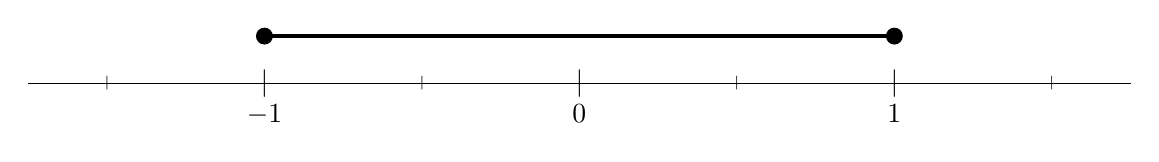
\begin{tikzpicture}[scale = 2]
\draw (-3.5,0) -- (0,0) -- (3.5,0);
\draw [very thick, black] (-2,0.3) -- (2,0.3);
\draw [fill = black] (-2,0.3) circle (0.5mm);
\draw [fill = black] (2,0.3) circle (0.5mm);
\draw (0,0) node {$|$} node [below = 1.5mm] {$0$};
\draw (1,0) node {\tiny$|$};
\draw (2,0) node {$|$} node [below = 1.5mm] {$1$};
\draw (3,0) node {\tiny$|$};
\draw (-1,0) node {\tiny$|$};
\draw (-2,0) node {$|$} node [below = 1.5mm] {$-1$};
\draw (-3,0) node {\tiny$|$};
\end{tikzpicture}
\end{center}
\bigskip
We can specify other sets in terms of absolute values. For example, the set of points with $|x| \geq 1$ is the union of two sets, $\set{x \mid x \leq -1} \cup \set{x \mid x \geq 1}$. On a number line this looks like
\bigskip
\begin{center}
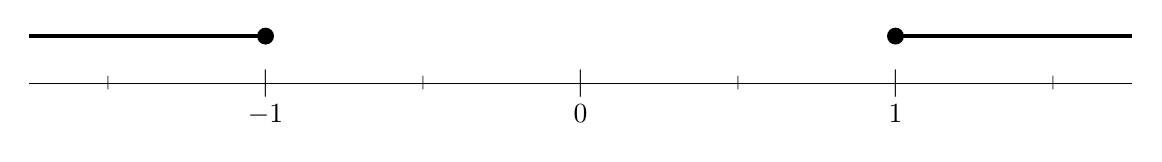
\begin{tikzpicture}[scale = 2]
\draw (-3.5,0) -- (0,0) -- (3.5,0);
\draw [very thick, black] (-2,0.3) -- (-3.5,0.3);
\draw [very thick, black] (2,0.3) -- (3.5,0.3);
\draw [fill = black] (-2,0.3) circle (0.5mm);
\draw [fill = black] (2,0.3) circle (0.5mm);
\draw (0,0) node {$|$} node [below = 1.5mm] {$0$};
\draw (1,0) node {\tiny$|$};
\draw (2,0) node {$|$} node [below = 1.5mm] {$1$};
\draw (3,0) node {\tiny$|$};
\draw (-1,0) node {\tiny$|$};
\draw (-2,0) node {$|$} node [below = 1.5mm] {$-1$};
\draw (-3,0) node {\tiny$|$};
\end{tikzpicture}
\end{center}